\section{ Experimental Results}\
\textcolor{red}{
Describe the setup of the experiments you ran, e.g., what evaluation metrics, datasets are used. Present the results, preferably in the form of tables and/or figures
}


\subsection{Dataset}

% Jayden

\subsection{Results}


\iffalse
We will conduct outdoor experiments on the top floor of the parking garage. Radar images (both 2D and 3D) will be collected with our custom-built Millimeter wave FMCW (Frequency Modulated Continuous Wave) radar system, operating around 60 GHz as shown in the figure above Both the radar transmitter and receiver antennas will be omni-directional. While the transmitter remains fixed, the receiver will move on a linear stage to synthesize a 1D or 2D antenna array to obtain the Direction of Arrival (DoA) measurement in a horizontal plane or the entire 3D space. We will first process raw radar data with fundamental radar signal processing algorithms, and filter out noise and unwanted interference to focus on only a few key features of the target. The target of interest can be either static or under motion. 

\subsection{Dataset Description}
The dataset we will create should include all significant features of a car. Therefore, we will place a car in a number of orientations in front of the radar, and try to filter out noise and interferences from other key points in preprocessing. We will also simulate the most likely relative positions and motions of the autonomous car with the radar system and other vehicles on the road, take a series of images as they move together.
\par We might have to face the problem of lack of accurate labels to our training set. One possible solution is to collect another set of reference data with cameras and train an additional neural network with well-developed vision models to label our radar images.

\begin{figure}
\centering
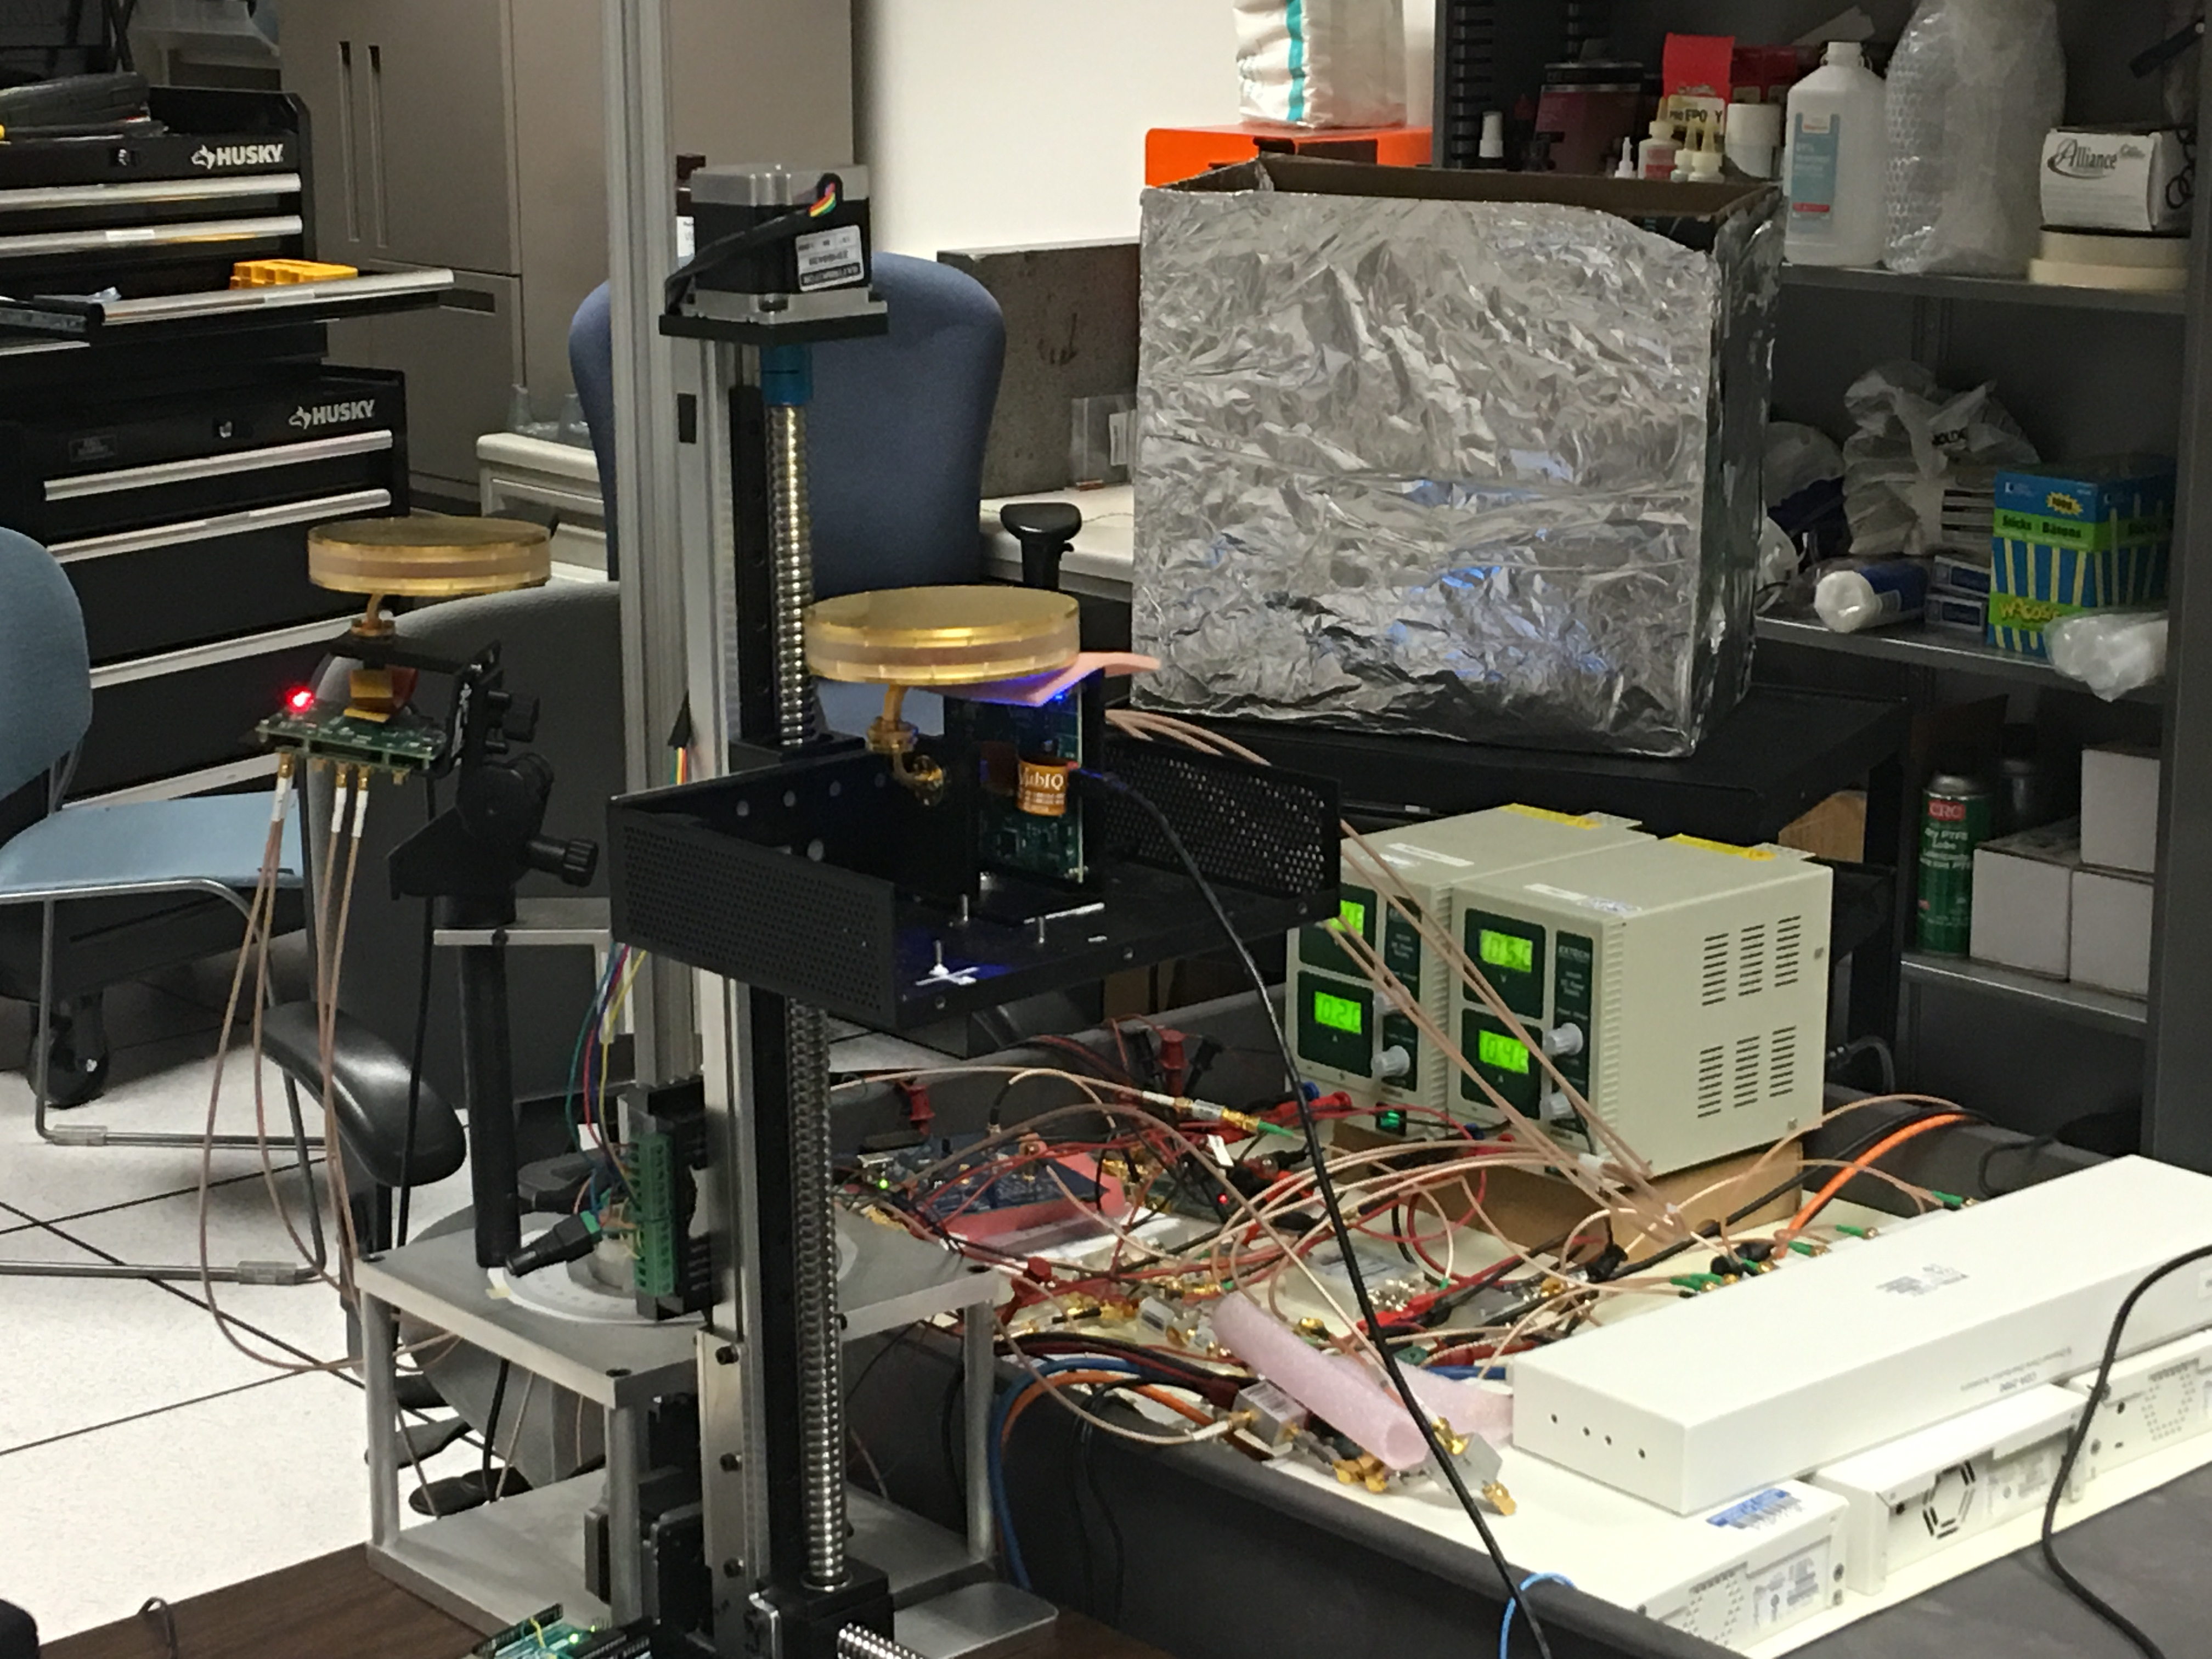
\includegraphics[width=8cm,height=6cm]{./figure/experiment_setup.jpg}
\caption{Custom-built 60 GHz mmWave radar imaging system}
\end{figure}

\fi
